% Kopfzeile beim Kapitelanfang:
\fancypagestyle{plain}{
%Kopfzeile links bzw. innen
\fancyhead[L]{\calligra\Large Vorlesung Nr. 10}
%Kopfzeile rechts bzw. außen
\fancyhead[R]{\calligra\Large 12.11.2012}
}
%Kopfzeile links bzw. innen
\fancyhead[L]{\calligra {\Large Vorlesung Nr. 10}}
%Kopfzeile rechts bzw. außen
\fancyhead[R]{\calligra \Large{12.11.2012}}
% **************************************************
%
%\setcounter{chapter}{4}
\chapter{Abbildungen und Funktionen}
\sS{Definition}
Seien $A, B$ Mengen. Eine Abbildung von $A$ nach $B$ ist eine Vorschrift, die jedem Element von $A$ ein Element von $B$ zuordnet.\\
\notat{$f: A \to B,\  a \mapsto f(a) \  a\in A$}
%
A heißt Definitionsbereich von $f$\\
B heißt Wertebereich von $f$
%
\bsp
\begin{enumerate}
\item {Alle Personen in $L1 \mapsto \N$\\
$P \mapsto$ Geburtsjahr von $P$}
%
\item{$f:\R → \R, \ f(x)=x^2$\\
$g:\R→\R_{\geq 0}=\{x\in\R|x\geq 0\}, \ g(x)=x^2$\\
$h: \R_{\geq 0} \to \R_{\geq 0} \ h(x) = x^2$}
\bem 
\item{
$f,g,h$ sind verschieden\\
Sei $M$ Menge. Die Identität von $M$ ist die Abbildung $id_{M}:M→M, \ id_M(x)=x$}
\end{enumerate}
%
\sS{Definition}
%
Eine Abbildung $f: A \to B$ heißt:
%
\begin{enumerate}
\item{\underline{injektiv} wenn gilt: Für alle $a, a' \in A$ mit $f(a) = f(a')$ ist auch $a = a'$}
\item{\underline{surjektiv} wenn gilt: Für jede $b\in B$ gibt es ein $a\in A$ mit $f(a)=b$}
\item{\underline{bijektiv} wenn $f$ injektiv und surjektiv ist}
\end{enumerate}
%
% Tafel 2.2
% Bild zeichnen
%
% Tafel 3.1
% Beispielbild
%
\bem
$f$ ist $\left\{
\begin{array}{c}
\text{injektiv}\\
\text{surjektiv}\\
\text{bijektiv}
\end{array}
 \right\}$ genau dann wenn für jedes $b \in B$ $\left\{\begin{array}{c} \text{höchstens}\\ \text{mindestens}\\ \text{genau} \end{array} \right\}$ ein $a \in A$ mit $f(a) = b$\\
%
\bsp
$f,g,h$ wie oben\\

\begin{description}
\item[f]{
\hspace{6mm}nicht surjektiv: es gibt kein $a\in\R$ mit $f(a)=-1$\\
nicht injektiv: $f(-2)=4=f(2), 2\neq -2.$}
%
\item[g]{
\hspace{5mm}ist surjektiv, denn für jedes $b \in \R_{\geq 0}$ gilt $f( \sqrt{b} ) = b$ also gibt es $b \in \R_a$\\
 ist nicht injektiv (wie $f$)}
%
\item[h]{
\hspace{5mm}surjektiv wie g. $(\sqrt{b} \geq 0)$\\
injektiv, denn: Wenn $a, a' \geq 0$ und $a^2 = (a')^2$ dann $a = a'$ also $h$ bijektiv.}
\end{description}
%
\sS{Definition}
Seien $f:A→B$, $g:B→C$ Abbildungen\\
Die Komposition von $f$ und $g$ ist die Abbildung\\
$g \circ  f: A→C$, $(g \circ f)(a):=g(f(a))$\\
Sprich $\circ$ "nach"
%
%
\sS{Satz} 
Eine Abbildung $f: A \to B$ ist bijektiv \equ \ es gibt eine Abbildung $g: B \to A$ mit $f \circ g = id_B$\\
(d.h. f(g(b)) = b für alle $b \in B$\\
      g(f(a)) = a für alle $a \in A$)\\
%
\sss{Definition} %ohne nummer
Wenn $f:A→B$ bijektiv ist, heißt die eindeutige Abbildung $g:B→A$ wie oben die Umkehrabbildung (inverse Abbildung) von $f$
Bezeichnung: $g=f^{-1}$.\\
%
\bew
Angenommen, $g: B \to A$ gegeben mit $f \circ g = id_B, g \circ f = id_A$ \footnote{Dies gilt, weil $g$ als Umkehrfunktion von $f$ definiert ist.}\\
$f$ surjektiv: Sei $b \in B$. $b = f(g(b)) = f(a)$ mit $a = g(b)$ \ok\\
$f$ injektiv: Sei $a, a'$ mit $f(a) = f(a')$ zeige $a = a'$ \\
$a = g(f(a)) = g(f(a')) = a' $\ok \\ \\
%
Angenommen, $f$ ist bijektiv, zeige $g$ existiert.\\
Gegeben sei $b \in B$ $f$ bijektiv $\Rightarrow$ es gibt genau ein $a \in A $ mit $f(a) = b$ 
Setze $g(b):=a$ Das definiert Abbildung $g:B→A$\\
Zeige $g \circ f=id; f \circ g = id$\\
$(f\circ g)(b)=f(g(b))=f(a)=b$ wobei $a$ wie eben\\ \\
%
Zeige: $(g \circ f) (a) $ für alle $a \in A$\\
$f$ injektiv: Reicht $f(g(f)a))) = f(a)$\\
Das gilt weil $f \circ g = id_B$ \ok \\ \\
Eindeutigkeit von $g$:\\
Angenommen, $g^* : B \to A$ erfüllt $g^* \circ f = id_A$,
$f \circ g^* = id_B$ \\
%
Dann gilt: $g=g\circ id_B=g\circ f\circ g^*=id_A\circ g^* = g^*$ \qed
\bsp
Bewiesen 5.12
\begin{itemize}
\item{$f: \R_{\geq 0} \to \R_{\geq 0}, f(x) = x^k$ bijektiv ($k \geq 1$)\\
Die Umkehrabbildung $f^{-1}$ heißt k-te Wurzelabbildung $f^{-1}(x) = \sqrt[k]{x}$ }
%
\item{exp: $\R→\R_{>0}$ $exp(x) = \sum_{k=0}^{\infty}$ (Absolutkonvergente Reihe) ist bijektiv. Die Umkehrabbildung heißt Logarithmus. bew.
$log = exp()^{-1} \R_{\geq } \to \R_a$ }
\end{itemize}
%
\section*{Bild und Urbild}
\sS{Definition}
Sei $f:A→B$ Abbildung\\
\begin{enumerate}
\item{Für eine Teilmenge $X \subset A$ ist \\
$f(x) := \{f(x) | x \in X\} \subseteq B$ \\
das Bild von $X$ unter $f$}
\item{Für eine Teilmenge $Y \subseteq B$ ist $f^{-1}:=\{a\in A|f(a)\in Y\}\subseteq A$ das Urbild von $Y$ unter $f$}
\end{enumerate}
\underline{\underline{Vorsicht}} nicht Urbild und Umkehrabbildung verwechseln.\\
\bsp
$f:\R→\R, f(x)=x^2$\\
$f(\{1, 2, -2\}) = \{1, 4\}$\\
$f^{-1}(\{1,-2,4\})=\{1,-1,2,-2\}=f^{-1}(\{1,4\})$\\
$f^{-1}(\{9\})=\{3,-3\} \\
f^{-1}(\{-5\})=\emptyset$
%
\section*{Funktionen}
\sS{Definition}
Sei $D\subseteq\R$ Teilmenge. Eine reelle Funktion auf $D$ ist eine Abbildung $f:D→\R$\\
%
Der \underline{Graf} von $f$ ist die Menge $\Gamma_f = \/(x, f(x) | x \in D \}$) \\
$ \Gamma_f \subseteq D \times \R$ 
%
\bem Oft ist $D$ ein Intervall
%
\sS{Definition Intervalle}
\begin{wrapfigure}{r}{0.2\textwidth}
  \begin{center}
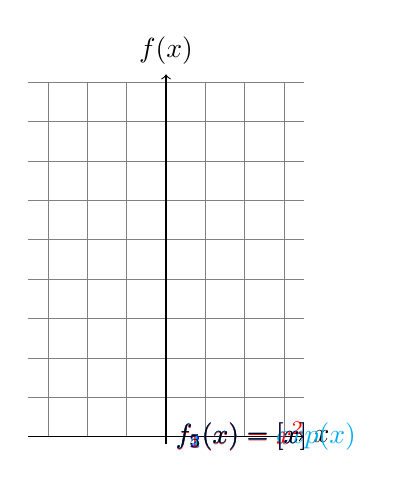
\begin{tikzpicture}[scale=.5, domain=-3:3, samples=2000]
    \draw[very thin,color=gray] (-3.5,-0.0) grid (3.5,9.0);
    \draw[->] (-3.5,0) -- (3.5,0) node[right] {$x$};
    \draw[->] (0,-0.2) -- (0,9.2) node[above] {$f(x)$};
    \draw[color=red] plot[id=abb1.1] function{x*x} 
        node[right] {$f_1(x) =x^2$};
    \draw[color=blue] plot[id=abb1.2] function{abs(x)} 
        node[right] {$f_2(x) = |x|$};
    \draw[color=cyan] plot[id=abb1.4] function{exp(x)} 
        node[right] {$f_4(x) = exp(x)$};
    \draw[color=black] plot[id=abb1.5] function{floor(x)} 
        node[right] {$f_5(x) = [x]$};
\end{tikzpicture}
  \end{center}
\end{wrapfigure}
seien $a, b \in \R$ \\
$[a, b] = \{x \in \R| a \leq x \leq b\}$ (abgeschlossen)\\
$(a, b] = \{x \in \R| a < x \leq b\}$ (halboffen)\\
$[a, b) = \{x \in \R| a \leq x < b\}$ (halboffen)\\ %mit klammer zu pberer zeile\\
$(a, b) = \{x \in \R| a < x < b\}$ (offen)\\
%
Uneigentliche Intervalle: \\
$[a, \infty) = \{x \in \R | a \leq x\} = \R_{\geq a}$\\
$(a, \infty) = \{x \in \R | a < x\} = \R_{> a}$\\
$(- \infty, a] = \{x \in \R | x \leq a\} = \R_{\leq a}$\\
$(- \infty, a) = \{x \in \R | x < a\} = \R_{< a}$\\
$(- \infty, \infty) = \R$\\
%
\Bsp{Funktionen}
\begin{enumerate}
\item{$f:[0,2]→\R, f(x)=x^2, \Gamma_f \leq [0,2] x\R$}
\item{Betragsfunktionen: $|\ |: \R→\R, x\mapsto|x|$
%noch mehr graphen aaaahahhahahah
}
An dieser Stelle fehlen noch Graphen.
\item{$g:\R\bs\{0\}→\R, g(x)=\dfrac{1}{x}$
%graph
Hier auch.
}
\item{$exp:\R→\R$.}
\item{[.] : $\R \to \R$ Gaußklammer\\
$[x] := max\{n \in \Z | n \leq x \}$
\bsp
$[5] = 5$\\
$[5,78] = 5$\\
$[-1,2] = -2$}
\item{Sei $h:\R→\R$ definiert durch $h(x)=\begin{cases}0\ wenn\ x\in\Q\\ 1\ wenn\ x\notin\Q\end{cases}$\\
$h(\sqrt{2}) = 1, h (\frac{3}{7}) = 0$}
\end{enumerate}
%
\sS{Definition (Rechnen mit Funktionen)}
Sei $D \subseteq \R , \ f,g: D→\R$ Funktionen auf D.\\
Definiere
\begin{itemize}
\item{$f+g: D \to \R$ durch $(f + g)(x) := f(x) + g(x)$}
\item{$(f \cdot  g) (x) = f(x) \cdot g(x)$}
\item{Für $a\in\R$ setze $a·f: D→\R, (a·f)(x):=a·f(x)$}
\item{Angenommen, $f(x) \neq 0$ für alle $x \in D$ \\
$$\frac{1}{f}: D \to R, \frac{1}{f}(x) := \frac{1}{f(x)} = f(x)^{-1}$$
\underline{\underline{Vorsicht}} nicht $\frac{1}{f}$ mit Umkehrbild oder Urbild verwechseln}
\end{itemize}
%
\sS{Definition}
\begin{itemize}
\item{Eine \underline{Polinomfunktion} ist eine Funktion der Form\\
$f: \R → \R,\ f(x) = a_n x^n+a_{n-1}x^{n-1}+…+a_0=\ds\sum_{k=0}^n a_k x^k $\\
wobei $a_0,…,a_n \in \R$ fest}s
%
\item{Seien $f, g : \R \to \R $ Polymonfunktionen
Sei $D = {x \in \R | g(x) \geq 0}\leadsto \dfrac{f}{g} : D \to , Rx \mapsto \frac{f(x)}{g(x)}$
Solche Funktionen heißen rationale Funktionen.
\bsp
$f:\R\bs\{0,1\}→\R, \ f(x)=\dfrac{x^7+5x^2}{x(x-1)}$}
\end{itemize}
\sS{Definition}
Seien $f: C \to \R, g: D \to \R$ Funktionen sodass $f(C) \subseteq D$
Eine Komposition von f und g ist 
%
$g \circ f : C \to \R$\\
$(g \circ f) \ (x) = g(f(x))$